\documentclass[conference]{IEEEtran}
\ifCLASSINFOpdf
  \usepackage[pdftex]{graphicx}
  \graphicspath{{../pdf/}{../jpeg/}}
  \DeclareGraphicsExtensions{.pdf,.jpeg,.png}
\else
  \usepackage[dvips]{graphicx}
  \graphicspath{{../eps/}}
  \DeclareGraphicsExtensions{.eps}
\fi
\usepackage{cite}
\usepackage{times}
\usepackage[cmex10]{amsmath}
\usepackage{algorithmic}
\usepackage{array}
\usepackage[tight,footnotesize]{subfigure}
\usepackage{fixltx2e}
\usepackage{url}
\usepackage{lipsum}

\begin{document}

% paper title
\title{Iterative MIMO Detection for Large Wireless MIMO Systems}

% author names and affiliations
\author{\IEEEauthorblockN{}}

\author{
\IEEEauthorblockN{Alexandre P. J. Dixneuf}
\IEEEauthorblockA{Student (Affiliations)}
\IEEEauthorblockN{Antoine Berthet}
\IEEEauthorblockA{Professor (Affiliations)}

% make the title area
\maketitle

\begin{abstract}
    \lipsum[1]
\end{abstract}

% Found this command online to force wey
\providecommand{\keywords}[1]{\textbf{\textit{Index terms---}}#1}
\begin{keywords}
\textbf{Term1, Term2, Term3, Term4, Term5, Term6, Term7, Term8, ...}
\end{keywords}

\IEEEpeerreviewmaketitle

\section{Introduction}
\lipsum[2]

\section{Background}

\subsection{Subesection 1}
\lipsum[3]\cite{ExampleBIB}

\subsection{Subsection 2}
\lipsum[4]

\section{Theory and Reasoning}
\subsection{Theory}
\lipsum[5]

\subsection{Reasoing}
\lipsum[6]

\subsection{Example Image}
\lipsum[7] \ref{fig:example}.
\begin{figure}[h!]
    \centering
    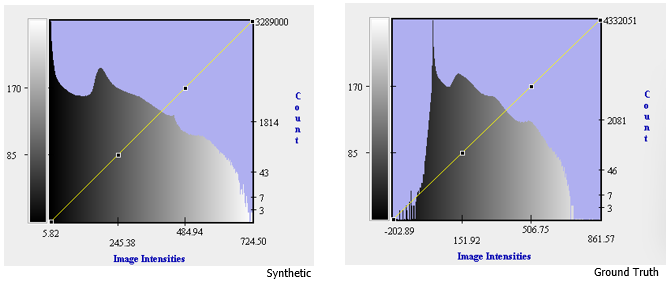
\includegraphics[width=0.30\textwidth]{Histogram Comparison.png}
    \caption{A side-by-side comparison of the intensity histogram between the post-processing synthesized T2w compared to the ground truth.}
    \label{fig:example}
\end{figure}

\section{Methods}
\lipsum[8]

\section{Experiments and Results}
\lipsum[9]

\section{Discussion}
\lipsum[10]

% References
\begin{thebibliography}{1}
\bibitem{ExampleBIB}
Gruszecki M, Lancaster G, Stefanovska A, Neary JP, Dech RT, Guminski W, Frydrychowski AF, Kot J, Winklewski PJ. \emph{Human Subarachnoid Space Width Oscillations in the Resting State}, 2018
\end{thebibliography}
\end{document}